
\documentclass[preprint]{aastex631}

\usepackage{subfiles}
\newcommand{\vdag}{(v)^\dagger}
\newcommand\aastex{AAS\TeX}
\newcommand\latex{La\TeX}
\usepackage{times}
\usepackage{enumitem}
\usepackage{subcaption}
\usepackage{tablefootnote}
\usepackage{multirow}
\usepackage{placeins}
\usepackage{float} 

% comment macros
\newcommand{\as}[1]{{\color{orange}[AS: #1]}}

\begin{document}

\title{Lunar Farside Technosignature \& Transients Telescope (LFT3)}

\author[0000-0003-3197-2294]{David R. DeBoer}
\affiliation{Sub-department of Astrophysics, University of Oxford, Oxford, OX1-3RH, UK}
\affiliation{Radio Astronomy Laboratory, University of California, Berkeley, CA, 94720 USA}
\author[0009-0009-3198-2768]{Charlie K. Ashe}
\affiliation{School of Physics, Trinity College Dublin, College Green, Dublin 2, Ireland}
\author[0000-0002-5927-0481]{Owen A. Johnson}
\affiliation{School of Physics, Trinity College Dublin, College Green, Dublin 2, Ireland}
\affiliation{Radio Astronomy Laboratory, University of California, Berkeley, CA, 94720 USA}
\author[0000-0002-4553-655X]{Evan F. Keane}
\affiliation{School of Physics, Trinity College Dublin, College Green, Dublin 2, Ireland}
\author[0000-0002-8455-9797]{Andrew C. Lesh}
\affiliation{Department of Civil and Environmental Engineering, Stanford University, CA, 94305 USA}
\author[0000-0003-3165-6785]{Steve Prabu}
\affiliation{Sub-department of Astrophysics, University of Oxford, Oxford, UK}
\author[0009-0008-0410-1833]{Kaia L. Reenock}
\affiliation{Haverford College, Dept. of Physics and Astronomy, Haverford, PA 19041 USA}
\author[0000-0002-8713-3695]{An\v{z}e Slosar}
\affiliation{Brookhaven National Laboratory, Physics Department, Upton, NY 11973 USA}
\author[0000-0002-4409-3515]{Chenoa D. Tremblay}
\affiliation{SETI Institute, 339 Bernardo Ave, Suite 200, Mountain View, CA 94043, USA}
\affiliation{Department of Physics and Astronomy, University of New Mexico, Albuquerque, NM 87131, USA}
\author[0000-0001-7836-1787]{Jake D. Turner}
\affil{Department of Astronomy and Carl Sagan Institute, Cornell University, Ithaca, New York 14853, USA}
\author[0000-0002-0387-6476]{Karl F. Warnick}
\affiliation{ECE Dept., Brigham Young University, Provo, UT, USA}
\author[0000-0003-2828-7720]{Andrew P. V. Siemion}
\affiliation{Sub-department of Astrophysics, University of Oxford, Oxford, UK}
\affiliation{SETI Institute, 339 Bernardo Ave, Suite 200, Mountain View, CA 94043, USA}
\affiliation{Berkeley SETI Research Center, University of California, Berkeley, CA, 94720 USA}
\author{Jamie Drew}
\affiliation{Breakthrough Initiatives, 6 Observatory St, Oxford OX2 6EW, UK}
\author{S. Pete Worden}
\affiliation{Breakthrough Initiatives, 9 Rue du Laboratoire, 1911 Gare Luxembourg, Luxembourg}



\begin{abstract}

We uniquely rely on radio telescopes to understand the bulk of baryonic matter in the Universe and the evolution of the Universe across cosmic time. There are two unavoidable limitations to our exploration of the cosmos with terrestrial-based radio telescopes: (1) the prevalence of interfering radio transmitters from human activity, and (2) the Earth's ionosphere and atmosphere, which are opaque or disruptive to many important frequency ranges.  Both limitations are ameliorated by reaching above the atmosphere and beyond Earth, a capability that, to date, has generally been the exclusive purview of expensive, government-funded space-based ``Great Observatories''. 

However, we are now on the cusp of a new era, with cost-effective access to space-- including the lunar surface-- becoming a reality. This will enable disparate groups to send instruments there, bringing about a transition from Earth-based observatories to space-based and cislunar telescopes. Although this shift provides exciting opportunities for new science, it will also introduce sources of radio frequency interference (RFI) to the quietest remaining location we have: the lunar farside. Although Earth- or Sun-orbiting telescopes allow for radio frequency measurements below the ionosphere cut-off, they are still exposed to RFI because Earth remains within their line of sight, even at vast distances. Until the Moon's farside becomes crowded with sources of artificial radio emissions, it offers a unique opportunity to measure radiation from the Universe with virtually no interference. The chance to make these measurements from the lunar farside before it is significantly affected by RFI is unparalleled in human history, but the window of opportunity is limited. Even in advance of any astronaut activity on the farside, multiple nations are planning constellations of Moon orbiting satellites for science, positioning, and relaying communications, which will inevitably pollute the farside's currently pristine radio environment.

We present here a proposed telescope covering 1 MHz -- 2.7 GHz that will land near the lunar antipode within five years to conduct baseline observations free from RFI. The Lunar Farside Technosignatures and Transients Telescope (LFT3) will search the farside sky for radio emissions from known and unknown sources, and create a historical record of lunar radio observations as the current silence gives way to a more crowded RF environment with the deployment of additional instruments. LFT3 is the {\em only} mission proposed to take advantage of this unique opportunity in human history.

%We will also discuss related activities for related ground-based and earth-orbiting instruments that will allow for prototyping and support of a lunar mission. 
%As a powerful tool for studying astrophysical processes, radio telescopes hold a prominent place in the astronomy community. There are two limitations to our exploration of the cosmos with terrestrial telescopes: the prevalence of radio transmitters in our daily lives and the ionosphere around the Earth, which creates a dispersion screen that is opaque over important frequency bands. We are, however, on the verge of overcoming these limitations by observing the cosmos from the moon. We are at a tipping point in having cost-effective access to space which will enable many nations to send experiments to the lunar surface and orbit and bring about a transition from Earth-based observatories to space-based telescopes. This provides opportunities for new science but will also bring radio frequency interference sources to the quietest remaining near-Earth location, the lunar farside. Until the moon's farside becomes crowded with sources of radio emission, the lunar farside offers a unique opportunity to measure radiation from the Universe with virtually no interference from radio waves. In this paper, we present an ultra high frequency (UHF) phased array telescope that will be landed near the lunar antipode within five years in order to conduct baseline observations free from radio frequency interference. The Lunar Farside Technosignatures and Transients Telescope (LFT3) will search the farside sky for radio emissions from known and unknown sources and create a historical record of lunar radio observations from the current pristine silence to a more crowded atmosphere as further instruments are deployed. The LFT3 is an opportunity never before offered in human history for the recording of signals in a completely silent environment. 



%Humanity is on the verge of being able to observe the cosmos from the moon with sufficient accuracy in order to gain a deeper understanding of astrophysical processes.  This necessitates a transition from earth-based observatories to space-based telescopes.  We are at a tipping point in having cost-effective access to space which will enable many nations to send experiments to the lunar surface and orbit. This provides opportunities for new science but will also bring RFI sources to the quietest remaining near-earth location. Until the moon also becomes crowded with sources of radio emission, the lunar farside offers a unique environment to measure radiation from the Universe with essentially zero radio frequency interference. We describe an ultra high frequency (UHF) phased array telescope to be landed near the lunar antipode within five years to conduct initial baseline observations in the absence of RFI. The Lunar Farside Technosignatures \& Transients Telescope (LFT3) will search the farside sky for radio emissions from known and unknown sources and create a historical record of lunar radio observations from the current pristine silence to a more crowded environment as further instruments are deployed. LFT3 is a once-in-human-history opportunity to record signals in a fully quiet environment. 

\end{abstract}

\section{Introduction} 
\label{sec:intro}
\subfile{introduction}

%\section{Lunar Farside}
%\label{sec:Lunar Farside Location Conditions}
%\subfile{farside}

\section{Science Case}
\label{sec:science}
\subfile{science_new}

%\section{Observing Within The Terrestrial RF Environment}
%\label{sec:rfenv}
%\subfile{terrestrial_rf}

\section{Payload and Operations}
\label{sec:payload}
\subfile{payload}

\section{Other Considerations}
\label{sec:otherconsiderations}
\subfile{other_considerations}



\section{Conclusion}

As the only proposed mission to exploit the singular opportunity for RFI-free astrophysical observations across HF, VHF, and UHF from the lunar farside, the LFT3 mission is uniquely positioned to redefine our understanding of the radio universe from this unique vantage point in space and time. In an environment quieter than even that in which the famed "Wow!" signal was detected, LFT3 offers an unprecedented chance to conduct technosignature searches with confidence and unambiguity never before possible in human history. Crucially, this opportunity is time sensitive. The lunar farside will soon face increasing RFI contamination as more missions are launched, and the timeline for the proposed LFT3 mission is uniquely aligned to capitalize on this fleeting window. Every signal detected by LFT3 in this pristine radio environment will have an unambiguous scientific value. In addition to technosignature searches, LFT3 is designed to discover previously undetected populations of low-dispersion radio transients, probing low-frequency phenomena inaccessible from Earth. The mission opens new frontiers in radio astronomy, including low-frequency Very Long Baselines Interferometry (VLBI) with Earth-based observatories and enables the first modern detection of low-frequency radio emission from the outer planets of our Solar System, last observed by Voyager. LFT3 represents a once-in-a-generation, time-critical opportunity to listen to the radio universe in a way that has never been possible before and, if missed now, will likely never come again.

%In view of the compelling opportunity for science observations offered by LFT3, and the value of creating a historical record of the electromagnetic environment on the lunar far side, we recommend that LFT3 be funded, developed, and launched by the end of 2029, prior to the saturation of cislunar space by governmental and commercial activity. Even when escaping the RF distortion caused by the Earth's atmosphere, any location with the Earth in its line of sight will be subject to terrestrial radio frequency interference.  Due to it always facing away from Earth, the lunar farside is currently the most radio-quiet environment that humans have access to.  As governmental and commercial activities ramp up in cislunar space, it is crucial that a mission measure baseline RF spectra from the lunar farside and conduct sensitive observations there before it becomes polluted with anthropogenic signals.  Before this unique window in human history closes, LFT3 will search for extraterrestrial technosignatures, transient phenomena (including solar emissions, planetary auroral emissions, pulsars, fast radio bursts, and long-period radio transients), and atomic spectral signatures (for studying extra-galactic hydrogen distribution and the cosmological structure of the Universe during the Cosmic Dark Ages).  Additional experimental payloads could help investigate the local lunar environment, including the composition of regolith at LFT3's remote landing site.

%More conventional missions using Earth-based telescopes, Earth-orbiting telescopes, or even Moon-orbiting telescopes simply won't be capable of continually performing such sensitive observations while simultaneously escaping the distortion of the Earth's atmosphere and the noise of terrestrial RFI.  LFT3 is uniquely enabled by the commercial space revolution, which offers dramatically lower launch costs than historic norms, and as of January 2025, provides transportation to the lunar surface.  This revolution, allowing affordable access to this radio-quiet environment for the first time, also spells its end.  If we do not move quickly, the opportunity to perform these observations from such a pristine environment will disappear forever and later missions to the lunar farside will not have access to any clean RF baseline measurements.  The time to act is now!

\newpage
\appendix
% \begin{landscape}

\section{Science Traceability Matrix}

\begin{figure}
    \centering
    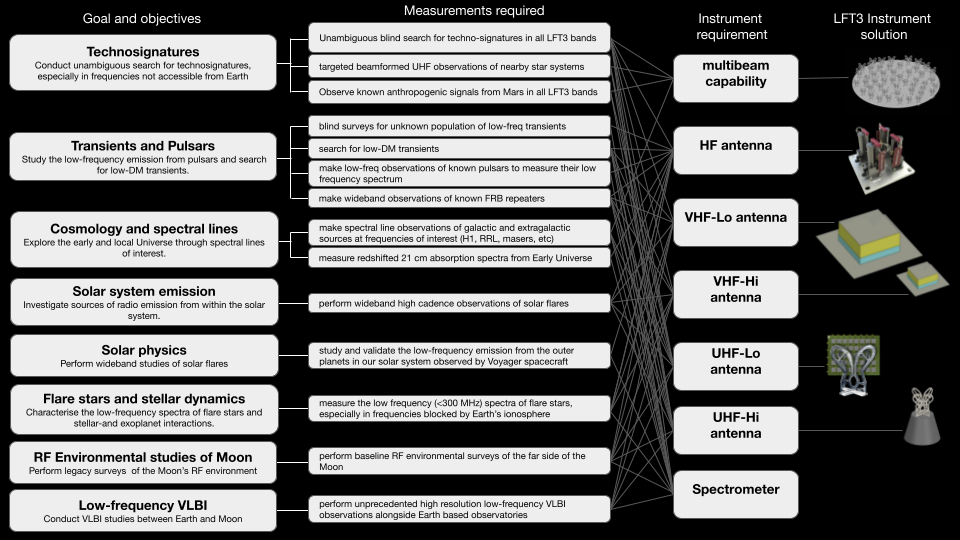
\includegraphics[width=1.2\linewidth, angle=90]{figures/ScienceTraceabilityMatrix.png}
    \caption{Science traceablity matrix for LFT3.}
    \label{fig:STM}
\end{figure}
    
% \end{landscape}

\newpage
\bibliography{bibs,bibfiles/radio-stars,bibfiles/transients,bibfiles/solarsystem-emission,bibfiles/solar}{}
\bibliographystyle{aasjournal}

\end{document}

